\section{Analysis} \label{analysis}

\subsection{Hate speech statistics}

After extracting all the features, we had a closer look at them to identify which features are characteristic for hate speech.
Firstly, the semantic features in general do not signify whether a post is hate speech or not. Neither the number of exclamation marks, question marks, full stop marks, interjections or all caps words show any sign of signifying hate speech. These features are evenly distributed regarding hate speech versus non-hate speech.
The only semantic features which indicate hate speech are the number of words and - to a very small degree - the number of laughing expressions.
As already mentioned in \autoref{sec:data_analysis} the more words a post consists of, the likelier it is to be classified as hate speech (illustrated in \autoref{fig:wordclouds}).
Although, there are only very few laughing expressions identified per post (most do not contain any), there is a tendency for hate speech posts to contain more laughing expressions, such as \enquote{haha}, \enquote{lol} or similar.

Slightly more telling is the topic feature we trained using LDA with only 2 topics. It seems to have somewhat trained to classify into hate and non-hate - as we hoped. The hate speech posts are more likely to be classified as topic 0 than non-hate speech posts. But this difference is not really significant.

A more interesting and characteristic feature seems to be sentiment-based. As described, we extracted a sentiment-score (polarity) for each post using vader and this clearly differentiates between hate speech and non-hate speech, as shown in \autoref{fig:statistics_sentiment}.
This shows, that a negative sentiment-score indicates a post being rather likely to contain hate speech. The more positive the sentiment-score is, the less probable it is classified as hate speech.

\begin{figure}[ht]
    \centering
    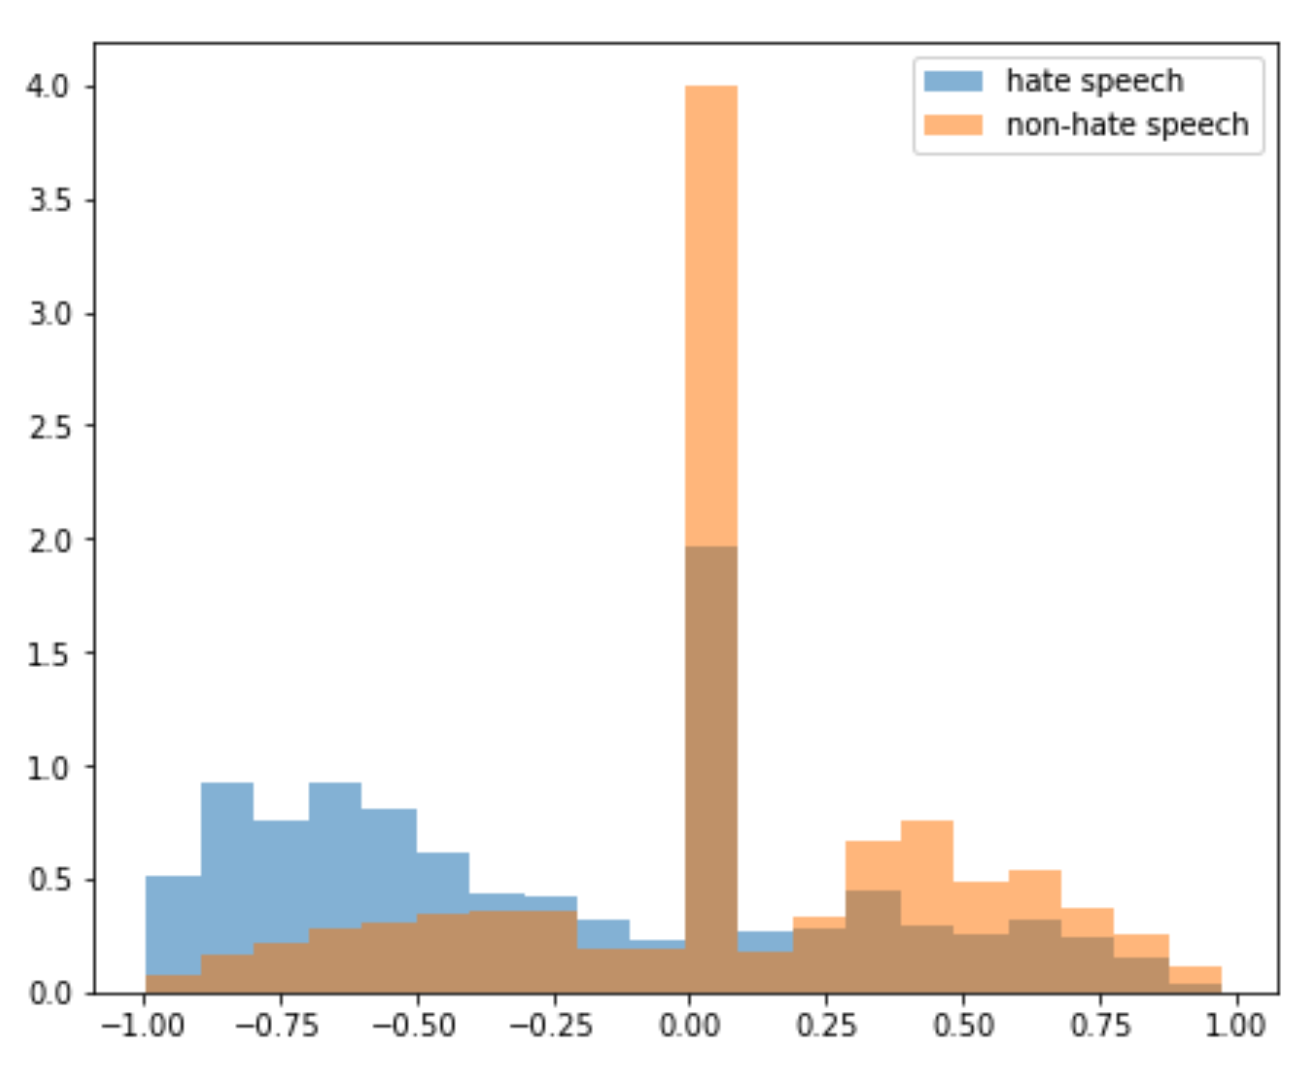
\includegraphics[width=0.7\linewidth]{figures/statistics_sentiment.png}
    \caption{Normalized distribution of sentiment score for hate speech vs. non-hate speech}
    \label{fig:statistics_sentiment}
\end{figure}

Further meaningful features were found using a dictionary approach by using the training data to generate a dictionary for hate speech and neutral words. The number of hateful words is distributed such that hate speech posts contain significantly more, whereas the number of neutral words does not differ much.
Examples for the most common hateful words found in hate speech posts are \enquote{fag}, \enquote{bitch}, \enquote{ass} or \enquote{nigga}. These words basically did not occur in non-hate speech posts. The most common neutral words are less informative, as the suffixes \enquote{ll} and \enquote{ve} are the most common ones for hate speech and non-hate speech posts.

Furthermore, we had an extensive look at unigrams, bigrams and trigrams for hate speech and these are significantly overrepresented in hate speech posts compared to non-hate speech posts. This especially holds true for the unigrams such as \enquote{white} which appears in 15\% of hate speech posts or \enquote{not} appearing in 9\% of hate speech posts. Both of these appear only half as often in non-hate speech posts.
The identified bigrams only show up in a very small percentage of posts, but significantly less in non-hate speech posts. Most common bigrams for hate speech are \enquote{white trash}, \enquote{look like} and \enquote{ass nigga}.

Lastly, the feature pattern-count can somewhat indicate hate speech, as the mean amount is higher for hate speech compared to non-hate speech. As one can see in \autoref{fig:statistics_pattern_count} hate speech tends to contain more patterns (which of course were trained by using the hate speech data).

\begin{figure}[ht]
    \centering
    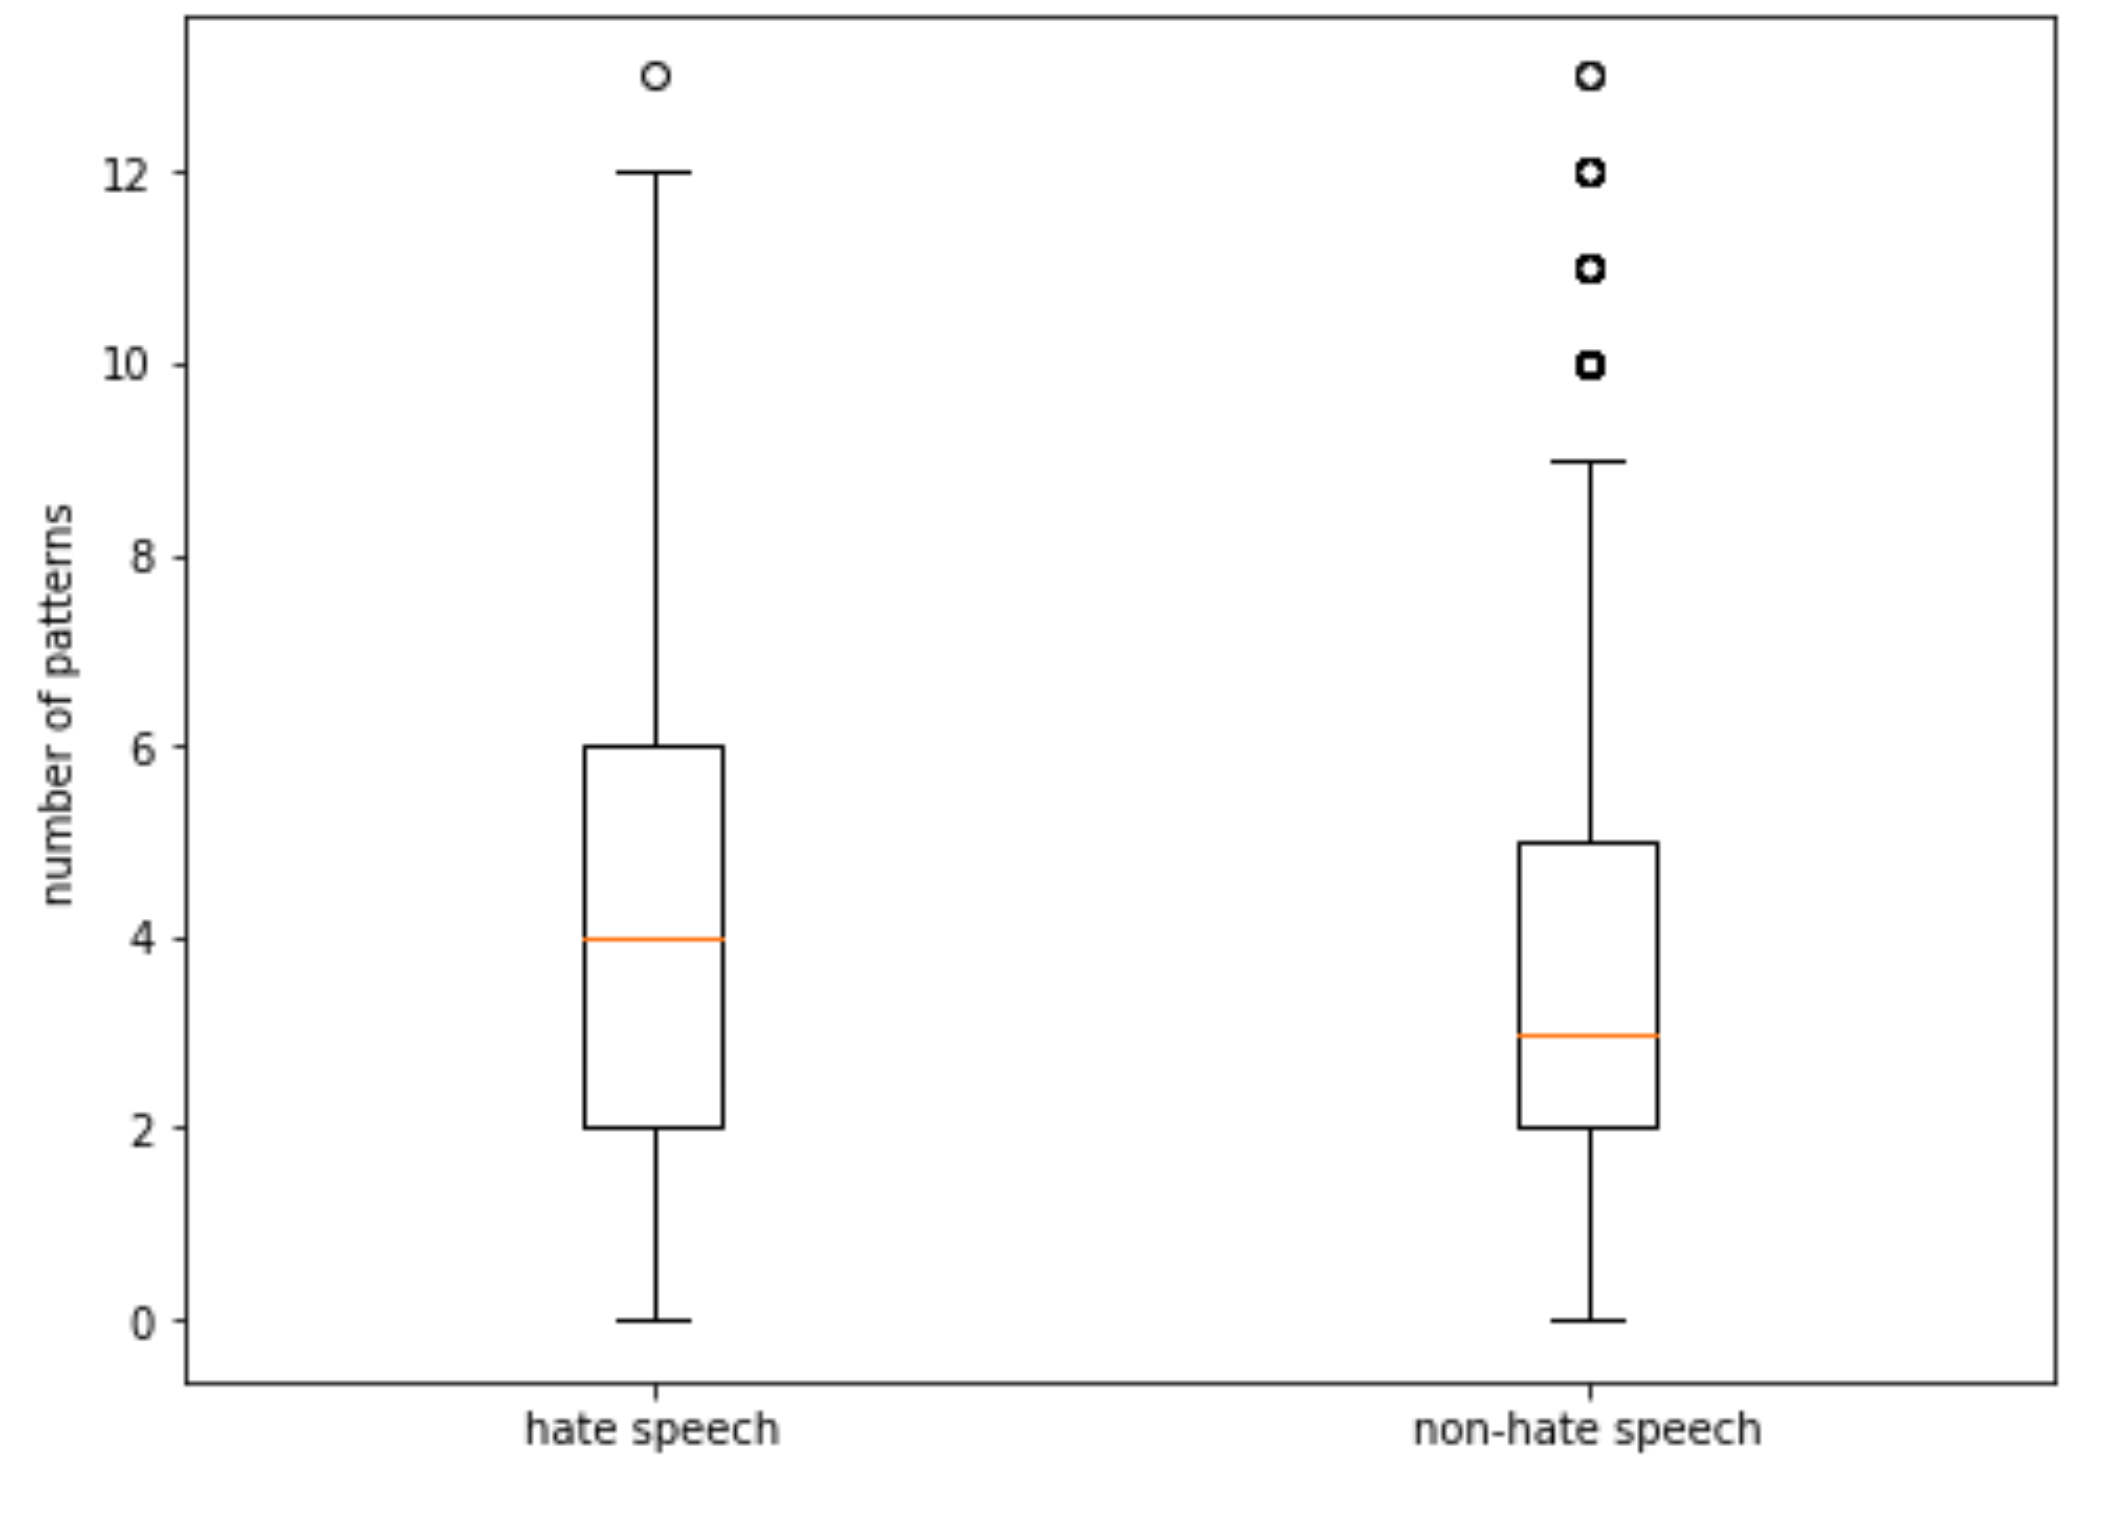
\includegraphics[width=0.7\linewidth]{figures/statistics_pattern_count.png}
    \caption{Boxplots comparing the number of patterns occurring in hate speech vs. non-hate speech}
    \label{fig:statistics_pattern_count}
\end{figure}

But maybe it would be worthwhile to have a closer look at the patterns and adjust them for some future work. Because when we look at single patterns, some occur more often in hate speech and some more often in non-hate speech (in our dataset). For example the pattern \enquote{adjective, noun (JJ, NN)} occurs in 56\% of hate speech and in 48\% of non-hate speech, whereas the pattern \enquote{determiner, noun} occurs in 5\% less hate speech posts than non-hate speech posts. So a more thorough analysis of these patterns could benefit this feature a lot, maybe by using individual features for each pattern. For example the biggest difference in occurrences is achieved by the pattern \enquote{personal pronoun, non-3rd person singular present verb (PRP, VBP)} with a 10\% difference.
